\documentclass[a4paper,12pt]{report}

\usepackage{graphicx} 

\begin{document}

\title{Curso práctico multiplataforma de Tratamiento Digital de la Imagen con Jupyter}
\author{ Ana Cuevas Bravo}
\maketitle

\newpage
\pagenumbering{roman}

\renewcommand{\abstractname}{Resumen}
\renewcommand{\chaptername}{Capítulo}

\begin{abstract}
Your abstract goes here...
...
\end{abstract}


\tableofcontents
\newpage
\pagenumbering{arabic}

\renewcommand{\abstractname}{Resumen}


\chapter{Introducción}


\chapter{Objetivos}
\section{Objetivos}
\section{Requisitos}
\section{Metodología}

\chapter{Infraestructura}

En esta sección se detallan tanto el software empleado para la realización del trabajo, como la estructura previa que existía en la asignatura y que ha servido como base para las nuevas prácticas. \\

 El lenguaje de programación utilizado ha sido Python, profundizaremos en las bibliotecas que tiene este lenguaje para el tratamiento de imagen que han sido necesarias para el desarrollo del trabajo. Esta sección también explicará en que consiste la plataforma Jupyter notebook y las ventajas que tiene en su uso para la docencia. Por último, se hablará de Matlab, la plataforma original que se usa en la asignatura de Tratamiento Digital de la Imagen y la estructura general que tienen las prácticas de esta asignatura.

\section{Python y tratamiento de imagen}

Python es un lenguaje de programación interpretado de alto nivel orientado a objetos creado en los años 80 por Guido van Rossum. Se caracteriza por tener una sintaxis sencilla, fácil de leer, lo que facilita el mantenimiento de programas y lo hace accesible para principiantes. Tiene una amplia biblioteca base y además permite el uso de módulos y paquetes. Al ser interpretado en lugar de compilado el proceso de debugging es más rápido.\\

 Python se está usando cada día más para el tratamiento de imagen, esto se debe a que es un lenguaje muy accesible, siendo gratuito y con una sintaxis sencilla. Con el tiempo han ido surgiendo bibliotecas específicas para el tratameinto de la imagen en Python como Pil (Python Imaging Library) también llamada Pillow, Scikit-image y Open-CV, esta última será la que más se use en este proyecto.\\

Otras bibliotecas que facilitan el tratamiento de imagen en Python son Numpy, una biblioteca para facilitar el uso de matrices y arrays en Python así como las funciones matemáticas relacionadas y Matplotlib que permite  la representación de datos en forma de gráficos.\\

\subsection{OpenCV}

Como ya hemos mencionado antes, OpenCV(Open Source Computer Vision Library) es una biblioteca centrada en el tratamiento de imagen y video (Computer Vision) y en aprendizaje de máquina, con interfaces para varios lenguajes de programación como C++, Python o Java. OpenCV es la biblioteca de procesamiento de imagen más usada en el mundo con más de 18 millones de descargas. Originalmente programada en C el resto de lenguajes usa diferentes interfaces para acceder al código. Esto permite mejorar el rendimiento siendo C el lenguaje más rápido en ejecución.\\

OpenCV contiene  desde funciones de bajo nivel para el procesado de imagen hasta algoritmos complejos para deteccion de caras. En este trabajo, ya que trata de dar una base de tratamiento de imagen, usaremos funciones de bajo nivel como filtros o funciones para cambiar de espacio de color.\\

En este trabajo se ha usado la versión 4.2.0 de OpenCV.\\

\subsection{Numpy}
\subsection{Matplotlib}
\subsection{Scikit-learn}	
\section{Jupyter}
\section{Matlab}
\section{Estructura de las prácticas de TDI}


Las prácticas originales para la asignatura de Tratamiento Digital de la Imagen consisten en una carpeta zip que se ponía a disposición de los alumnos en el aula virtual de la asignatura. Dentro de esta carpeta están las imágenes que se van a utilizar en la práctica (cuando no eran imágenes internas de MatLab), funciones adicionales necesarias en caso de que no existieran previamente y un enunciado en pdf. En la imagen \ref{carpetapracticas} se puede ver un ejemplo de una de estas carpetas.
\begin{figure}[h]
\centering
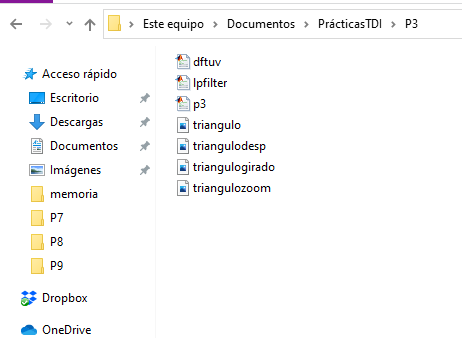
\includegraphics[width=0.5\textwidth]{carpetapracticas}
\caption{ejemplo de carpeta de prácticas}
\label{carpetapracticas}
\end{figure}

Las prácticas se realizaban en hora de clase en uno de los laboratorios de Windows del campus. Se podían realizar enteras en la duración de la clase. \\

La profesora daba una breve explicación inicial sobre el tema de la práctica, siempre relacionado con lo que se hubiera dado en las clases de teoría recientes, el resto de la práctica se podía seguir de forma libre con el enunciado, con la profesora respondiendo las dudas que surgieran en el desarrollo del ejercicio. \\

Los enunciados son instrucciones detalladas sobre los pasos a seguir para realizar la práctica, con poco o nada de teoría ya que se asume que el alumno ha recibido las clases de teoría previas. El alumno debe crear un nuevo documento en Matlab e ir ejecutando paso a paso lo que pide el enunciado. \\

Los enunciados suelen comenzar con un breve párrafo explicando el objetivo de la práctica, por ejemplo en la práctica 4 que trata el tema de segmentación de Imagen la introducción dice: "El objetivo de esta práctica es comenzar a familiarizar al alumno con las herramientas básicas de segmentación de imagen en entorno MATLAB. Para ello se trabajará con la imagen en escala de
grises ‘calculadora.tif’, que acompaña al material de esta práctica. "\\

A partir de esta breve introducción la práctica suele estar dividida en secciones normalmente relacionadas con diferentes puntos tratados en la teoría y como llevarlos a cabo.\\

Los pasos a seguir en MatLab, por lo general, vienen dados en el enunciado que indica qué función usar y cómo llamar a las diferentes variables para mantener una consistencia en los nombres a lo largo de la práctica. En algunos casos se indica las variables necesarias para llamar a la función que se va a usar en esa sección del ejercicio, mientras que en otros se pide al alumno que use el comando \textsl{+help} para informarse sobre el funcionamiento de la función. Del mismo modo si, una función requiere de un valor a decidir, dependiendo de lo que se quiera conseguir con su uso, unas veces se da con el enunciado y otras se deja a criterio del alumno para que pruebe como cambian los resultados con diferentes variables y cuál sería la mejor solución para el problema planteado.\\

Otra característica común de los enunciados de TDI son las preguntas para responder, aunque no se pide una memoria en sí de las prácticas en los enunciados hay preguntas con el objetivo de que el alumno se plantee las respuestas y las razones de los pasos que se han ido realizando durante el ejercicio.  La siguiente imagen \ref{preguntasp4} muestra un ejemplo de estas preguntas del principio de la práctica 4.

\begin{figure}[h]
\centering
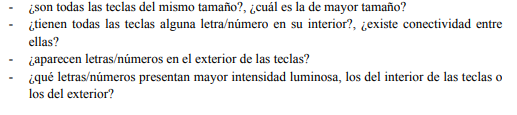
\includegraphics[width=1\textwidth]{preguntasp4}
\caption{ejemplo de preguntas realizadas en los enunciados de TDI}
\label{preguntasp4}
\end{figure}

Algunos de los enunciados tienen imágenes del aspecto que tendría que tener la imagen sobre la que se está trabajando después de ciertos pasos para que el alumno pueda ver si el ejercicio progresa adecuadamente o si debería modificar alguna variable o revisar el código.\\

Si se pide un algoritmo un podo más complejo en los enunciados aparece dado un trozo de ese código como ejemplo o directamente para copiar en matlab ya que el objetivo de estas prácticas no era aprender a programar en MatLab si no ilustrar de forma práctica lo dado en teoría de la asignatura.\\

Las prácticas se sulen centrar en el tratamiento de una imagen en específico, elegida para ilustar el tema del que trata la práctica, por ejemplo en la práctica 1 en el apartado que trata sobre color se scoge una imagen con diferentes verduras que muestran una variedad de colores para ilustrar la mezcla aditiva de color al representarse individualmentelas matrices de cada color del sistema de representación RGB. Debido a que algunas de las imágenes usadas en las prácticas originales pertenecen a Matlab o se desconoce su origen se ha tenido que buscar imágenes nuevas, siempre intentando mantener las características de la imagen original.\\

En total la asignatura consiste de nueve prácticas, 7 de imagen y 2 de video. \\

\chapter{Prácticas de TDI}

\chapter{Conclusiones}

\end{document}